%%%Variables

%%%
\question[20] A uniform-density disk of mass $M=12$ kg and radius $R=20$ cm is spinning about its central axis with angular speed $\omega=30$ rad/sec. A second disk, which is initially not rotating, is then dropped onto the first disk. Friction between the two disks causes the upper disk to begin rotating, and very quickly both disks are rotating together with the same angular speed. What is the final angular speed $\omega_f$, if the second disk has a radius $r=12$ cm, and a mass $m=4$ kg?

\begin{center}
	\begin{tabular}{cc}
		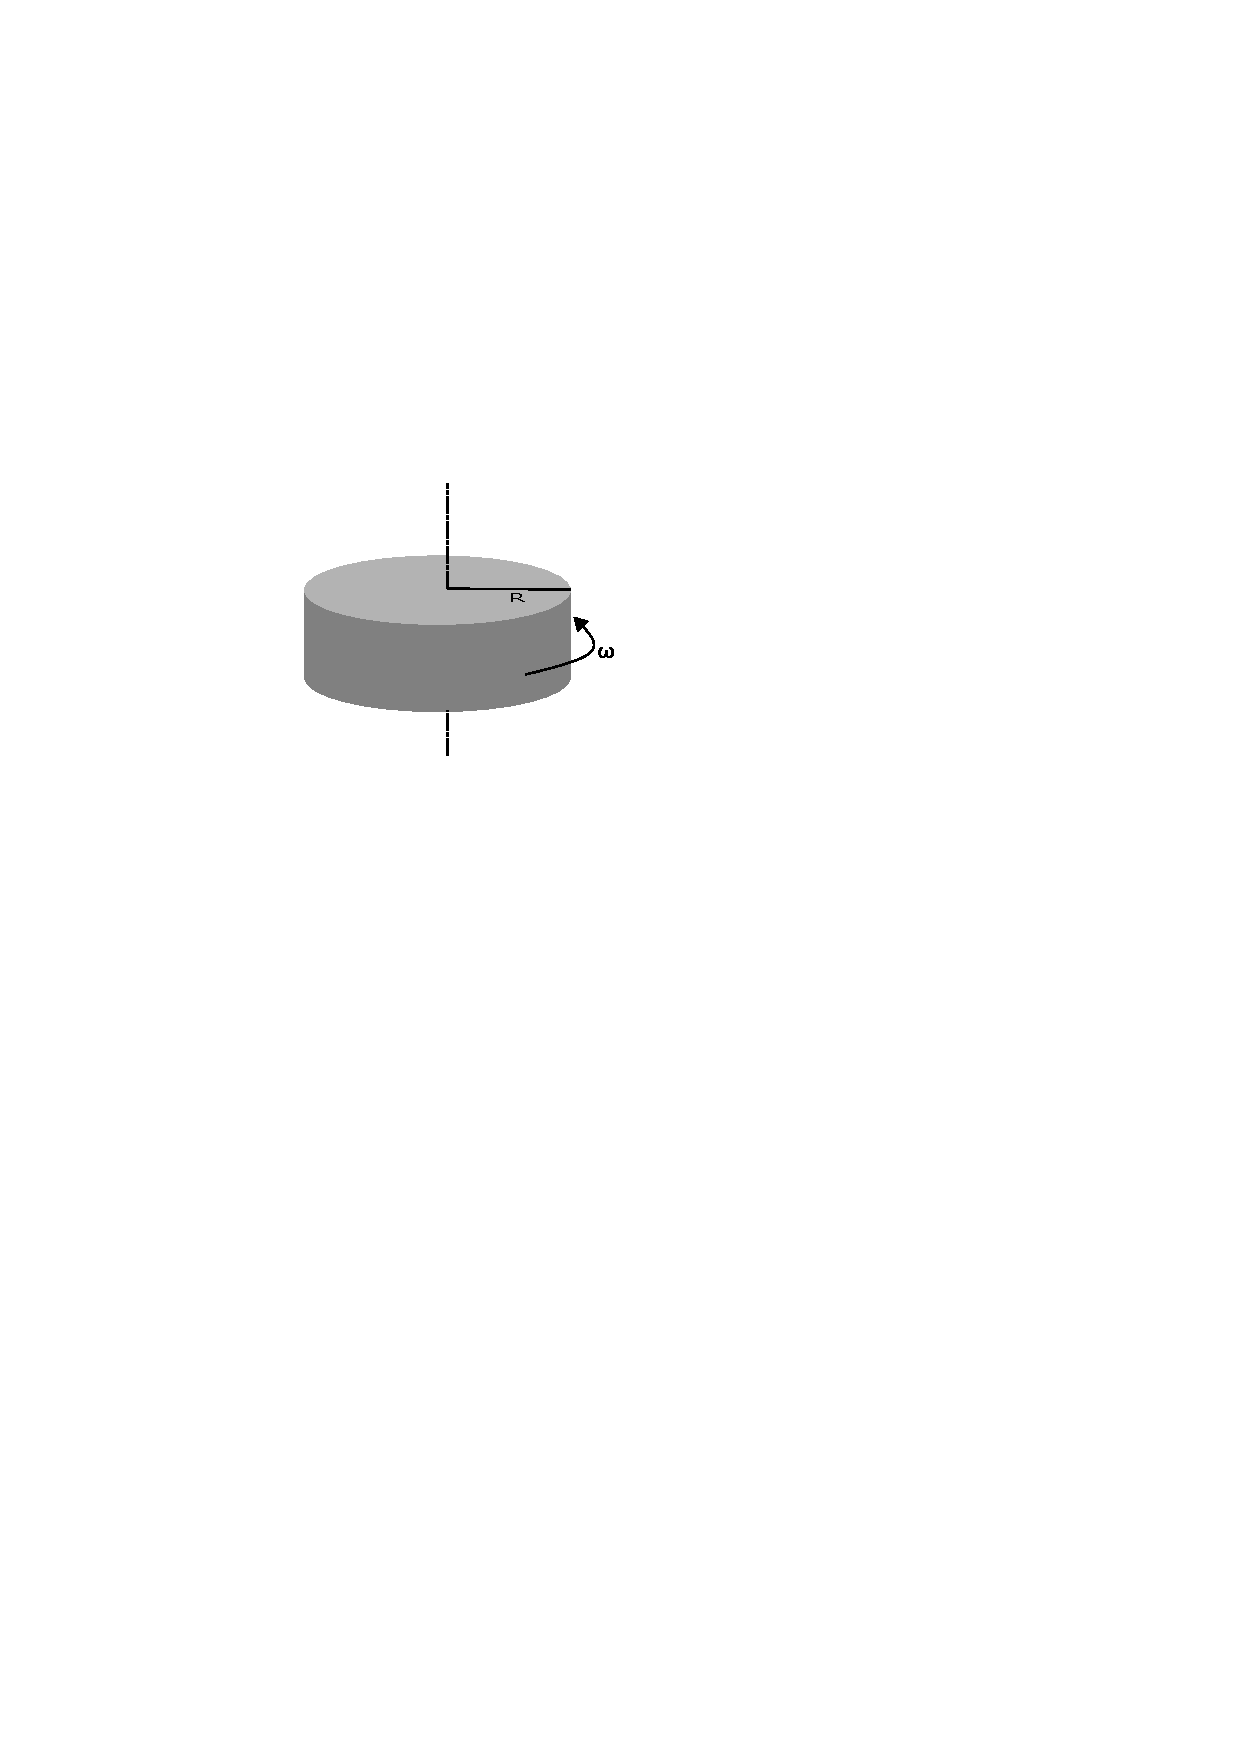
\includegraphics[trim=4cm 4cm 9cm 8cm]{disk1}&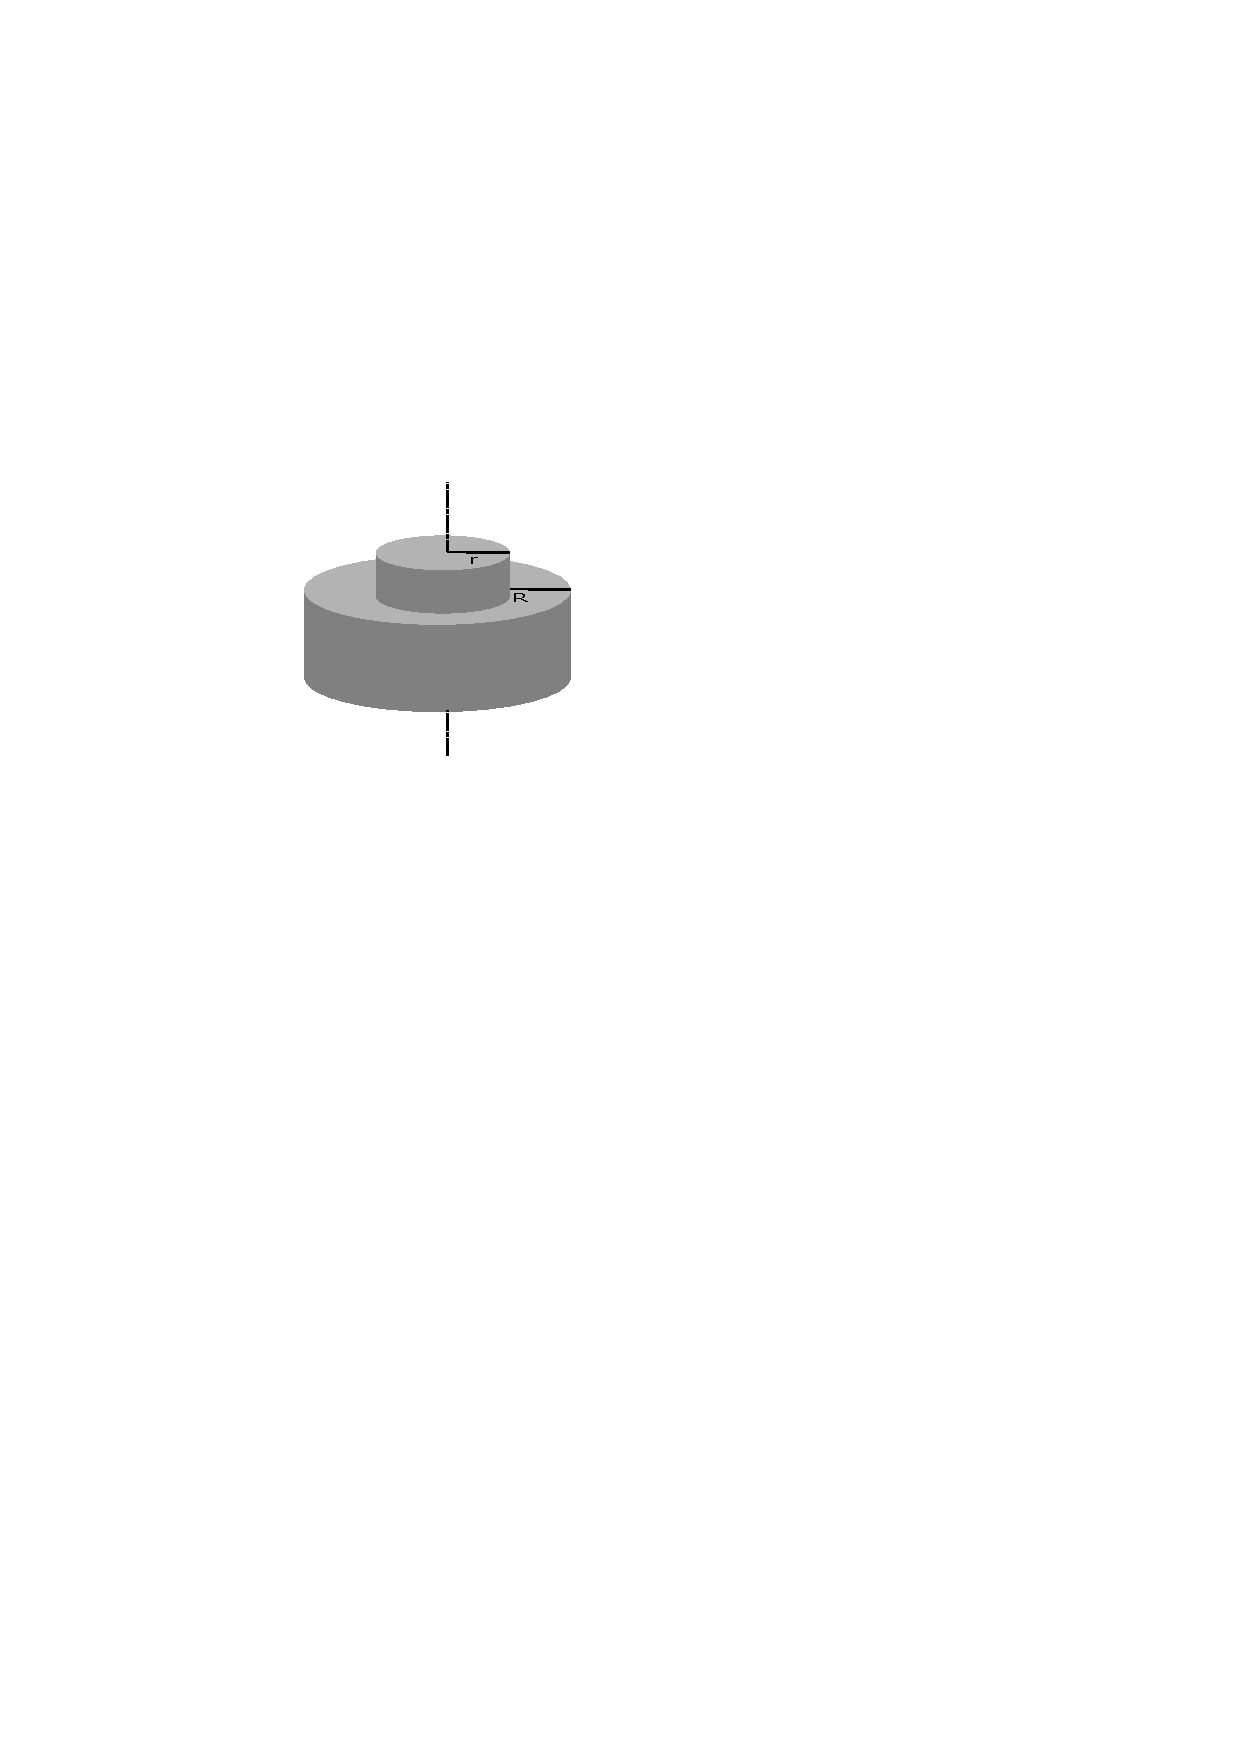
\includegraphics[trim=4cm 4cm 9cm 8cm]{disk2}
	\end{tabular}
\end{center}